% Hier wird der theoretische Teil vorgenommen. 

\chapter{Stand der Technik}


\section{Ähnlichkeitsmaße}

Im Folgenden sollen Ähnlichkeitsmaße zwischen Mengen, insbesondere 
solche, die als Kostenfunktion bzw. Bewertungsmetrik für einen binären 
Klassifikator verwendet werden können, untersucht werden. Hierzu wird zunächst Cross-Entropy betrachtet,
gefolgt von dem Dice- bzw. F-Maß. Weiter werden \ac{IoU} und das darauf aufbauende Quality-Maß betrachtet.

\subsection{\acf{BCE}}

Die \textit{Cross-Entropy} (bzw. dt. \textit{Kreuzentropie}) ist ein Maß des Unterschieds zweier
Wahrscheinlichkeitsdistributionen. Im Spezialfall einer binären Wahrscheinlichkeitsvariable 
kann die Cross-Entropy zur \textit{\acf{BCE}} spezialisiert werden, um auf ein binäres 
Klassifikationsproblem angewandt zu werden. 
\autoref{eq:bce} zeigt die Kalkulation von \ac{BCE}, wobei $p \in [0;1]$ die Prediction 
eines binären Klassifikators und $y \in {0,1}$ der Wert des Labels darstellen.
\begin{align}
	\label{eq:bce} BCE = -[p \cdot \log(y) + (1-p) \cdot \log(1-y) ]
\end{align} 
Um über $n$ Prediction-Label-Paare $(p_i; y_i)$ den \ac{BCE} zu berechnen, wird das arithmetische Mittel nach
\autoref{eq:bce-mean} gebildet \cite[S.~82]{Cybenko.1999}[S.~57--59]{Murphy.2012}.
\begin{align}
	\label{eq:bce-mean} BCE = -\frac{1}{n}\sum_{i = 1}^{n}[p_i \cdot \log(y_i) + (1-p_i) \cdot \log(1-y_i) ]
\end{align}

Im Sinne einer differenzierbaren Kostenfunktion im Kontext von \ac{ML} sind \ac{BCE},
\textit{negative Log-Likelihood} und \textit{Logistic-Regression} synonym \cite[S.~249]{Murphy.2012}. 

Aus \autoref{eq:bce-mean} geht hervor, warum \ac{BCE} gut geeignet für Klassifikationsprobleme ist.
Im Gegensatz zum mittleren absoluten Fehler, bei dem ein Fehler linear eingeht, und zum mittleren quadratischen Fehler,
bei dem ein Fehler quadratisch eingeht, geht ein Fehler bei \ac{BCE} exponentiell ein. 
Ein größerer Fehler wiegt also exponentiell stärker als ein kleinerer Fehler. 
Hierdurch werden die Fehler pro Datenpunkt und Klasse sehr klein, 
wodurch gute Performance und gute Generalisierung bei \ac{ML}-Modellen erreicht werden können. \\

Bei stark ungleichmäßiger Klassenverteilung kann es jedoch dazu kommen, 
dass die unterrepräsentierte Klasse kaum noch geschätzt wird, 
da der Fehler einer falsch geschätzten überrepräsentierten Klasse zu stark bestraft wird.
Dadurch lernt der Algorithmus, die unterrepräsentierte Klasse kaum zu schätzen.
Eine Abhilfe dagegen schafft eine Gewichtung der unterschiedlichen Klassen \cite[S.~4]{Ronneberger.18052015}.

\subsection{Dice- und F-Maß}

Das \textit{Dice-}, oder auch \textit{Sorensen-Dice-}Maß $D$ wurde 1945 bzw. 1948 erstmals vorgestellt und genutzt, um die Ähnlichkeit zweier botanischer Stichproben zu ermitteln. Verallgemeinert auf diskrete Mengen $X$, $Y$ kann deren Ähnlichkeit nach Dice $D$ beschrieben werden durch \autoref{eq:dice-coeff}. Es gilt $D \in [0; 1]$ \cites[S.~33]{Srenson.1948}[S.~297]{Dice.1945}. 
\begin{align}
	\label{eq:dice-coeff} D = \frac{2 \cdot | X \cap Y |}{2 \cdot | X \cap Y | + |Y \setminus X| + |X \setminus Y|} 
	=\frac{2 \cdot | X \cap Y |}{|X| + |Y|}
\end{align} 

Angewandt auf boolesche Mengen und binäre Klassifikatoren ist das Dice-Maß gleich dem $F_1$-Maß, das ein Maß für die Qualität eines statistischen Tests darstellt. Dafür sei $X$ nun die Menge der positiven Elemente und $Y$ die Menge der als positiv eingestuften Elemente. Dann ist die \textit{Genauigkeit} oder auch \textit{Precision} gegeben durch
\begin{align}
	\label{eq:precision} precision = \frac{|X \cap Y|}{|Y|}
\end{align}
der Anteil der richtig eingestuften Elemente an allen positiv eingestuften Elementen und die \textit{Trefferquote} oder auch \textit{Recall} gegeben durch
\begin{align}
	\label{eq:recall} recall = \frac{|X \cap Y|}{|X|}
\end{align}
der Anteil der richtig eingestuften Elemente an allen positiven Elementen. \\
Das F-Maß, bzw. genauer das $F_1$-Maß, ist dann gegeben durch das harmonische Mittel aus Precision und Recall, wobei $tp$ die Anzahl von wahr-positiven, $fp$ die Anzahl von falsch-positiven und $fn$ die Anzahl von falsch-negativen Elementen ist \cite{YutakaSasaki.2007}:
\begin{align}
	\label{eq:f1} F_{1} = \frac{2\cdot precision \cdot recall}{precision + recall} = \frac{2\cdot tp}{2 \cdot tp + fp + fn}
\end{align}
Precision und Recall können mit einem Faktor $\alpha$ unterschiedlich zueinander gewichtet werden, um mit $F_{\alpha}$ unterschiedliche Aspekte zu fokussieren. 

Das Dice-, bzw. $F_{\alpha}$-Maß kann leicht für eine differenzierbare Kostenfunktion genutzt werden mit Dice-Loss $D_{L}(X, Y) = 1 - D(X,Y)$, bzw. $F_{\alpha}$-Loss $F_{\alpha L}(X,Y) = 1 - F_{\alpha}(X,Y)$. 


\subsection{\acf{IoU}}

Die \textit{\acf{IoU}-} bzw. \textit{Jaccard-Ähnlichkeitsmetrik} ist ein weit verbreitetes Maß zur Bestimmung der Ähnlichkeit zwei diskreter Mengen. Hierzu seien $X$ und $Y$ diskrete Mengen. Dann ist die $IoU$ gegeben durch 
\begin{align}
	\label{eq:iou} IoU = \frac{|X\cap Y|}{|X \cup Y|} = \frac{| X \cap Y |}{| X \cap Y | + |Y \setminus X| + |X \setminus Y|}~.
\end{align} 
Für ein binäres Klassifikationsproblem lässt sich die $IoU$ ausdrücken durch 
\begin{align}
	\label{eq:iou-binary} IoU = \frac{tp}{tp + fp + fn}~,
\end{align}
wobei $tp$, $fp$, $fn$ wie in \autoref{eq:f1} \cite{Fletcher.2018}. 

Auffällig ist die Ähnlichkeit zum Dice- bzw. $F_{1}$-Maß. Es ist allerdings anzumerken, dass bei Dice/$F_1$ die $tp$, also die wahr-positiven, stärker gewichtet werden, als bei der \ac{IoU}. Die augenscheinliche Ähnlichkeit lässt sich durch die Beziehungen
\begin{align}
	\label{eq:dice-iou} IoU = \frac{D}{2 - D} \\
	D = \frac{2 \cdot IoU}{1 + IoU}
\end{align}
beschreiben.
Im Gegensatz zur \ac{IoU} wird beim Dice-Maß eine höhere Gewichtung auf die wahr-positiven Elemente 
gelegt.

\subsection{Quality}

Bei der \textit{Quality} handelt es sich um eine gepufferte Form des \ac{IoU},
die toleranter bezüglich der Lokalität der Elemente der verglichenen Mengen, oder konkreter,
der Pixel einer semantischen Segmentierung, ist, 
wobei für dieselbe Eingabe $Quality \geq IoU$; $Quality \in [0;1]$ gilt, abhängig von der Puffergröße. 
Die Quality wird analog zur \ac{IoU} über eine gepufferte Precision - die \textit{Correctness} - 
und über einen gepufferten Recall - die \textit{Completeness} - berechnet. \\
Die Quality soll einige Probleme der \ac{IoU} beheben, um ein Ähnlichkeitsmaß darzustellen, 
was näher an der praktischen und vom Menschen wahrgenommen Leistung eines \ac{ML}-Modells liegt.
So soll relativiert werden, dass vor allem im Randbereich einer Segmentierung einzelne abweichende Pixel
nicht als falsch anerkannt werden, sodass die Segmentierung im Großen und Ganzen als richtig anerkannt wird \cite{ChristianWiedemann.1998}. 


\section{Graphentheorie}

Dieser Abschnitt wird grundlegende graphentheoretische Begriffe definieren, die Darstellung in Computersystemen diskutieren, sowie einige einfache Algorithmen anführen, die für die weitere Arbeit relevant sind.

\subsection{Definitionen}


\textbf{Teilgraph} \\
Sei $G = (V, E)$ ein Graph. $T = (V', E') \subseteq G$ mit $V' \subseteq V$ und $E' \subseteq \{\{x,y\} \in E \mid x, y \in V'\}$ heißt \textit{Teilgraph} von $G$ ~\cite[S.~4]{Diestel.2016}.  


\textbf{Eingangs- und Ausgangsgrad im Digraph} \\
Sei $G = (V, E)$ ein Digraph und $v \in V$ ein Knoten in $G$, dann heißt $d^-_G(v) = | \{(x, y) \in E \mid y = v\} |$ der \textit{Eingangsgrad} von $v$ und $d^+_G(v) = | \{(x, y) \in E \mid x = v\} |$ der \textit{Ausgangsgrad} von $v$. Im klaren Kontext kann die Indizierung mit dem Graphen weggelassen werden. Knoten $v$ mit $d^-(v) = 0$ heißen  \textit{Quellen} und Knoten $v$ mit $d^+(v) = 0$ heißen  \textit{Senken} ~\cite[S.~460]{Satyanarayana.2014}.

\textbf{Pfade} \\ 
Ein \textit{Pfad} ist ein nicht-leerer, gerichteter Graph $P = (V, E)$ der Form $V = \{x_0, x_1, ..., x_k\};~E=\{(x_0,x_1), (x_1, x_2), ..., (x_{k-1}, x_k)\}$ wobei alle $x_i$ paarweise verschieden sind. Die Knoten $x_0$ und $x_k$ heißen \textit{Endknoten} (bzw. \textit{Start-} und \textit{Endknoten} im Digraph) und sind \textit{verbunden} durch $P$ ~\cite[S.~6]{Diestel.2016}. Pfade lassen sich auch als Folge ihrer aufeinander folgenden Knoten schreiben: $P = x_0x_1...x_k$ ~\cite[S.~7]{Diestel.2016}~\cite[S.~475]{Sedgewick.1992}. 


\textbf{Zyklen} \\
Sei $P = x_0...x_{k-1}$ ein Pfad und $k \geq 3$, dann ist der Graph $C := P + x_{k-1}x_0 = x_0...x_{k-1}x_0$ ein \textit{Zyklus} ~\cite[S.~8]{Diestel.2016}~\cite[S.~475]{Sedgewick.1992}.


\textbf{Transitive Hülle eines Knotens} \\
Sei $G = (V, E)$ ein Graph und $v \in V$ ein Knoten in $G$. Im Kontext
 dieser Arbeit sei die \textit{transitive Hülle eines Knotens} $v$ definiert
  als der Teilgraph $v^*_G := (V_v, E_v) \subseteq G$ 
  mit $V_v = \{x \in V \mid \exists P \subseteq G: P=x...v\}$ 
  und $E_v = \{ (x,y) \in E \mid x,y \in V_v \}$. 
  Also der Teilgraph in $G$, der alle Knoten und dazugehörigen Kanten enthält, von denen $v$ erreichbar ist. Es handelt sich bei dieser Definition also um einen \enquote{umgekehrten Erreichbarkeits-Teilgraph} ~\cite[S.~41--42]{Sandner.01.09.1998}.



\subsection{Tiefensuche (DFS)}

\autoref{code:dfs} zeigt eine Implementation der Funktion zur rekursiven Tiefensuche in C++ mit Adjazenzlisten als Graphrepräsentation. Hierbei ist \code{adj} ein Feld mit den (Adjazenz-)Listen und \code{visited} ein Array, welches jedem Knoten die Markierung ob er schon besucht wurde zuweist.

\lstinputlisting[
	label=code:dfs,    % Label; genutzt für Referenzen auf dieses Code-Beispiel
	caption=Rekursive Implementation der Tiefensuche mit Adjazenzlisten in C++. (In Anlehnung an \cite{GeeksforGeeks.2012}.),
	captionpos=b,               % Position, an der die Caption angezeigt wird t(op) oder b(ottom)
	style=EigenerCppStyle,   % Eigener Style der vor dem Dokument festgelegt wurde
	firstline=1,                % Zeilennummer im Dokument welche als erste angezeigt wird
	lastline=8                 % Letzte Zeile welche ins LaTeX Dokument übernommen wird
]{Quellcode/dfs.cpp}


\section{Submodelle} \label{sec:submodelle}

Die Submodelle werden durch die \ac{ProdDeco} aus dem (Haupt-)Modell des Szenarios erstellt. Dabei wird für \ac{SNP} und \ac{SOP} gleichermaßen verfahren. 

\subsection{Elementtypen} \label{sec:elements}
Das Modell eines Szenarios beinhaltet Elemente mit verschiedenen Elementtypen, wovon die wichtigsten im Folgenden vereinfacht vorgestellt werden:

\begin{itemize}
\item \textit{Quota Arrangement} - Ein vordefiniertes Kontingent an Materialbezug bzw. Materialverteilung, welches während des Optimierungslaufs strikt eingehalten werden muss \cite{.20220812c}. \\ Ein Beispiel wäre hierfür: Es werden 100 Stück von Produkt P1 an Lokation L1 benötigt. Es bestehen folgende Quota Arrangements: \begin{itemize}
\item Genau 40\% des Bedarfs müssen über einen Transport von Lokation L2 gedeckt werden.
\item Mindestens 10\% müssen über einen Transport von Lokation L3 gedeckt werden.
\item Genau 20\% müssen von einer Produktion in L1 gedeckt werden.
\end{itemize} 
\item \textit{Ressource} - Ein lokations-gebundenes Asset mit begrenzter Kapazität, welches eine bestimmte Funktion in der Supply Chain erfüllt. Die Ressource gehört zu genau einer Lokation, aber ihre Kapazität kann auf mehrere Produkte aufgeteilt werden. Beispiele: Eine Maschine, eine Person, ein Lager oder ein Transportmittel \cite{.20220812b}.
\end{itemize}

\section{Ähnlichkeitsmaße zwischen Graphen in der Literatur} \label{sec:sim_lit}

Im Folgenden wird eine Auswahl an Ähnlichkeitsmaßen zwischen Graphen aus der Literatur vorgestellt.

\subsubsection{Azyklischer Graph Edit Distance} \label{sec:sim_edit_dist}

Die \textit{Azyklischer Graph Edit Distance} beschreibt die minimale Anzahl an elementaren Veränderungen (Einfügen, Löschen, Umbenennen von Knoten), die durchgeführt werden müssen, um aus einem azyklischen (ungerichteten) Graph einen anderen zu machen \cite{Zhang.1989}. Hierbei wird allerdings rein die Ähnlichkeit der Struktur ermittelt.

\subsubsection{Similarity Flooding} \label{sec:sim_flooding}

Beim \textit{Similarity Flooding} wird die initiale Ähnlichkeit zweier Elemente aus zwei zu vergleichenden Graphen berechnet und diese Ähnlichkeit dann per Fixpunktiteration an benachbarte Knoten propagiert \cite{S.Melnik.2002}. Es läuft also unter der Annahme, dass aus dem Finden zweier ähnlicher Elemente eine Ähnlichkeit für die Nachbarelemente folgt. 

\subsubsection{Similarity of Weighted Directed Acyclic Graphs} \label{sec:sim_dag}

Sei $G = (V, E)$ ein \ac{DAG}. \textit{Similarity of Weighted Directed Acyclic Graphs} beschreibt einen Algorithmus zur effizienten Bestimmung der Ähnlichkeit von weighted \acp{DAG} \cite{Jin.2004}.
 
\begin{figure}
	\centering
	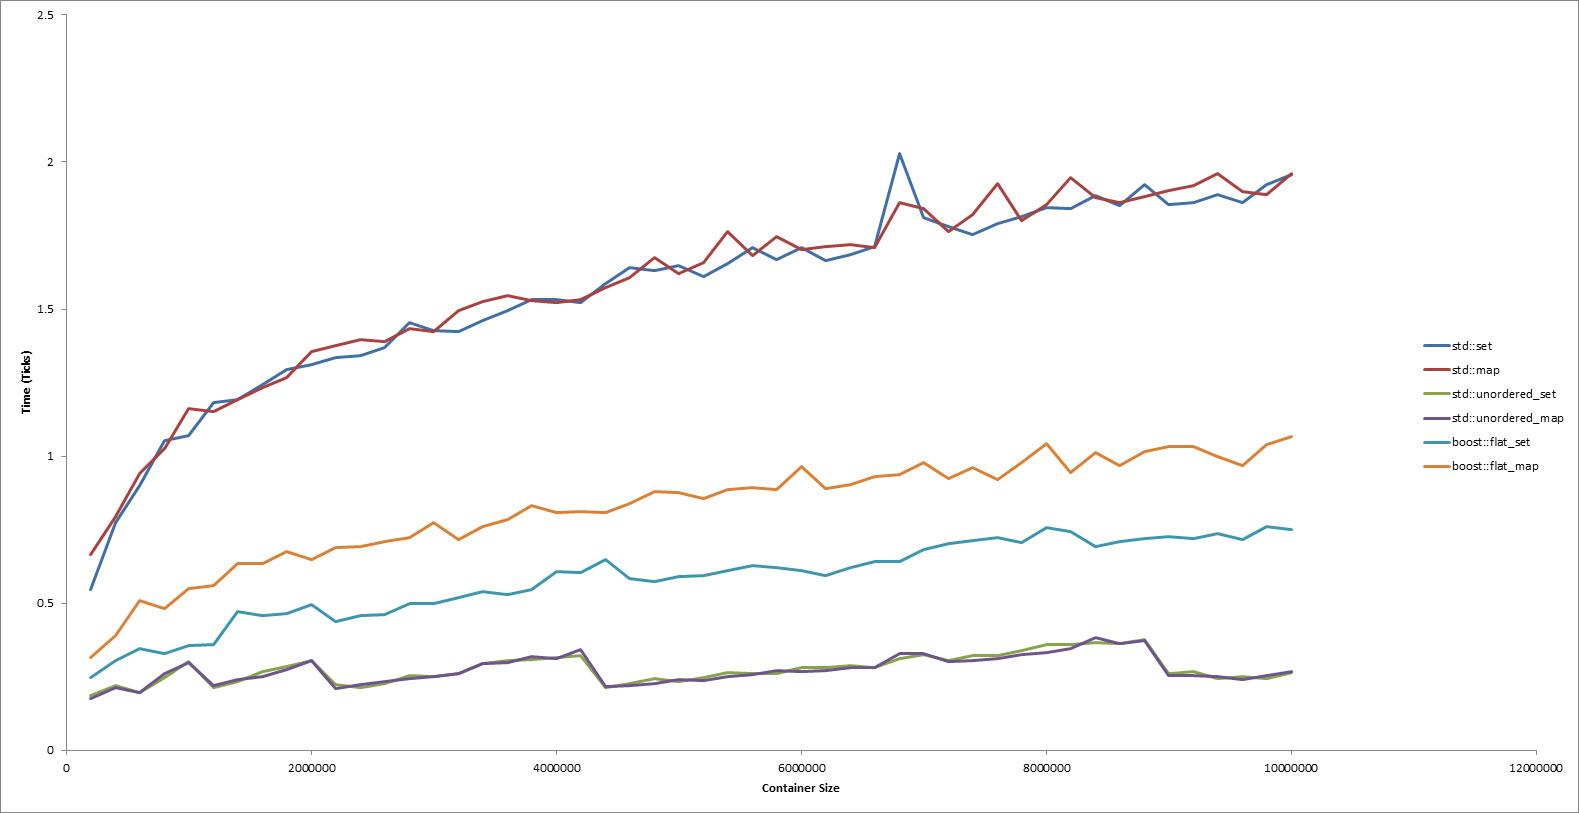
\includegraphics[width=\textwidth]{Bilder/GCC_timings_10M.jpg} 
	\caption{Lookup-Performanceunterschiede zwischen Map (rot), Set (blau), Flat\_Map (gelb), Flat\_Set (hellblau), Hash-Map (violett), Hash-Set (grün). Abszisse: Container-Größe 0, 2 Mio., ..., 12 Mio. Ordinate: Time in Ticks.\\ Flat\_X ist herbei ein sortierter Vektor \cite{.20220811}.\\ (Abb. entnommen aus \cite{.20220819b}.)}
	\label{fig:container_perf}
\end{figure} 
